\section{Experiment}
We conducted the frame per second (FPS) experiment\footnote{https://github.com/ZJUVAG/NetV.js/tree/benchmarks/benchmarks} to test the rendering performance of our \name with other popular tools and libraries which are supports network rendering, including D3-SVG, D3-Canvas, Cytoscape.js, Sigma.js (WebGL), and Stardust.js. In particular, \name, Sigma.js, and Stardust.js use WenGL to render data. To simulate real-world network data, we set the density of the network as 20, it means the ratio of the number of edges to the number of nodes is 1 to 20. The display refresh rate is 144Hz, the GPU is GTX 1060 with 6G.


From the line chart (\autoref{fig:eva}), \name, Stardust.js, and D3-Canvas can render around 100,000 elements. Our \name can render more than 1 million elements with FPS greater than 1.

\begin{figure}[htbp]
    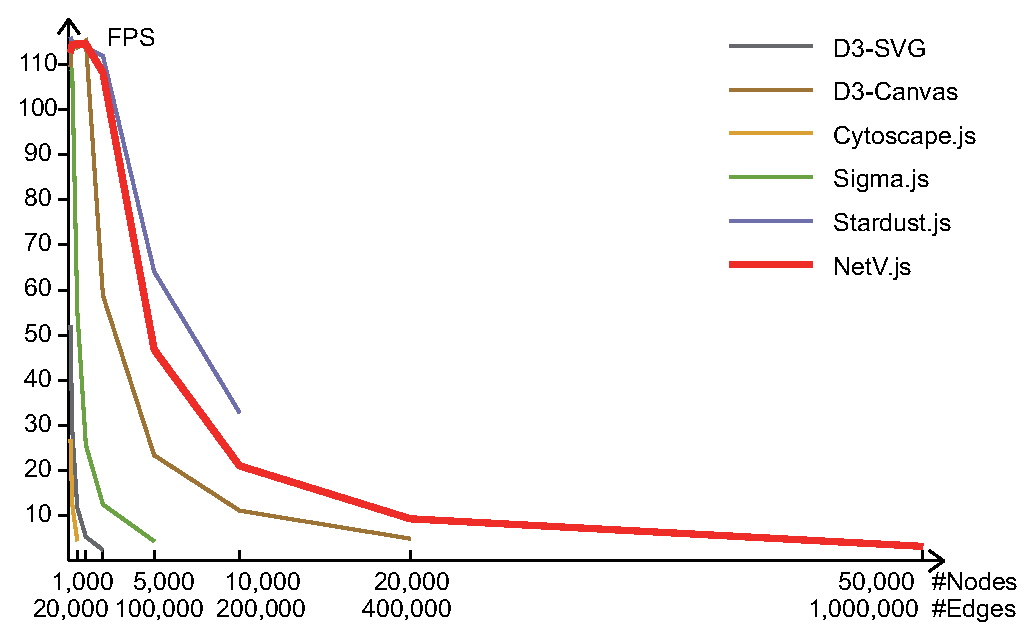
\includegraphics[width=\linewidth]{fig/eva.eps}
    \caption{
        The Frame per Second (FPS) experiment.
    }
    \label{fig:eva}
\end{figure}